\chapter{Architectures}

Finding a suitable architecture is a vital step in creating a well-performant deep learning model. By leveraging different techniques, we balance introduction of inductive biases and possibility for complexity, which hopefully can help us end up with a generalizing model.

\section{Recurrent Neural Network}

The \gls{RNN} is a standard architecture when it comes prediction on sequence data. It has been tried and tested, showing promising results for audio tasks.

The fundamental building block for \gls{RNN}s is the \textit{recurrent unit}. It iterates the whole input sequence, storing information from previous timesteps in a form of memory, through maintenance of a \textit{hidden state}. This can be extended to gaining information about future timesteps by using \textit{bidirectional} versions. In this way, prediction on current timesteps are affected by the information from surrounding timesteps. This is relevant in tasks such as \gls{ADT} as auditory information usually spreads over several timesteps, e.g. the timbre of an instrument event lingering after onset.

\begin{figure}[H]
    \centering
    \usetikzlibrary{positioning, chains, shapes.geometric, fit, shapes, arrows.meta, calc, backgrounds}

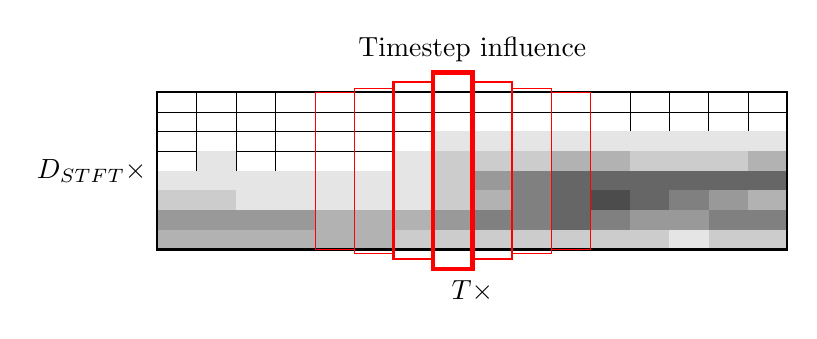
\begin{tikzpicture}[
    very thick,
    arrow/.style={
        -latex,
        very thick,
        rounded corners=0.2cm
    },
    ]

% ------ Grid ------

\draw[transform canvas={xscale=2}, step=0.25cm, ultra thin] (-2, 1) grid (2, 3);
\node[anchor=south] at (0, 3.25) {Timestep influence};
\node[anchor=east] at (-4, 2) {$D_\text{STFT}\times$};
\node[anchor=north] at (0, 0.75) {$T\times$};

% ------ Values ------

\fill[black!30] (-4.0, 1.0) rectangle (-3.5, 1.25);
\fill[black!30] (-3.5, 1.0) rectangle (-3.0, 1.25);
\fill[black!30] (-3.0, 1.0) rectangle (-2.5, 1.25);
\fill[black!30] (-2.5, 1.0) rectangle (-2.0, 1.25);
\fill[black!30] (-2.0, 1.0) rectangle (-1.5, 1.25);
\fill[black!30] (-1.5, 1.0) rectangle (-1.0, 1.25);
\fill[black!20] (-1.0, 1.0) rectangle (-0.5, 1.25);
\fill[black!20] (-0.5, 1.0) rectangle (0.0, 1.25);
\fill[black!20] (0.0, 1.0) rectangle (0.5, 1.25);
\fill[black!20] (0.5, 1.0) rectangle (1.0, 1.25);
\fill[black!20] (1.0, 1.0) rectangle (1.5, 1.25);
\fill[black!20] (1.5, 1.0) rectangle (2.0, 1.25);
\fill[black!20] (2.0, 1.0) rectangle (2.5, 1.25);
\fill[black!10] (2.5, 1.0) rectangle (3.0, 1.25);
\fill[black!20] (3.0, 1.0) rectangle (3.5, 1.25);
\fill[black!20] (3.5, 1.0) rectangle (4.0, 1.25);
\fill[black!40] (-4.0, 1.25) rectangle (-3.5, 1.5);
\fill[black!40] (-3.5, 1.25) rectangle (-3.0, 1.5);
\fill[black!40] (-3.0, 1.25) rectangle (-2.5, 1.5);
\fill[black!40] (-2.5, 1.25) rectangle (-2.0, 1.5);
\fill[black!30] (-2.0, 1.25) rectangle (-1.5, 1.5);
\fill[black!30] (-1.5, 1.25) rectangle (-1.0, 1.5);
\fill[black!30] (-1.0, 1.25) rectangle (-0.5, 1.5);
\fill[black!40] (-0.5, 1.25) rectangle (0.0, 1.5);
\fill[black!50] (0.0, 1.25) rectangle (0.5, 1.5);
\fill[black!50] (0.5, 1.25) rectangle (1.0, 1.5);
\fill[black!60] (1.0, 1.25) rectangle (1.5, 1.5);
\fill[black!50] (1.5, 1.25) rectangle (2.0, 1.5);
\fill[black!40] (2.0, 1.25) rectangle (2.5, 1.5);
\fill[black!40] (2.5, 1.25) rectangle (3.0, 1.5);
\fill[black!50] (3.0, 1.25) rectangle (3.5, 1.5);
\fill[black!50] (3.5, 1.25) rectangle (4.0, 1.5);
\fill[black!20] (-4.0, 1.5) rectangle (-3.5, 1.75);
\fill[black!20] (-3.5, 1.5) rectangle (-3.0, 1.75);
\fill[black!10] (-3.0, 1.5) rectangle (-2.5, 1.75);
\fill[black!10] (-2.5, 1.5) rectangle (-2.0, 1.75);
\fill[black!10] (-2.0, 1.5) rectangle (-1.5, 1.75);
\fill[black!10] (-1.5, 1.5) rectangle (-1.0, 1.75);
\fill[black!10] (-1.0, 1.5) rectangle (-0.5, 1.75);
\fill[black!20] (-0.5, 1.5) rectangle (0.0, 1.75);
\fill[black!30] (0.0, 1.5) rectangle (0.5, 1.75);
\fill[black!50] (0.5, 1.5) rectangle (1.0, 1.75);
\fill[black!60] (1.0, 1.5) rectangle (1.5, 1.75);
\fill[black!70] (1.5, 1.5) rectangle (2.0, 1.75);
\fill[black!60] (2.0, 1.5) rectangle (2.5, 1.75);
\fill[black!50] (2.5, 1.5) rectangle (3.0, 1.75);
\fill[black!40] (3.0, 1.5) rectangle (3.5, 1.75);
\fill[black!30] (3.5, 1.5) rectangle (4.0, 1.75);
\fill[black!10] (-4.0, 1.75) rectangle (-3.5, 2.0);
\fill[black!10] (-3.5, 1.75) rectangle (-3.0, 2.0);
\fill[black!10] (-3.0, 1.75) rectangle (-2.5, 2.0);
\fill[black!10] (-2.5, 1.75) rectangle (-2.0, 2.0);
\fill[black!10] (-2.0, 1.75) rectangle (-1.5, 2.0);
\fill[black!10] (-1.5, 1.75) rectangle (-1.0, 2.0);
\fill[black!10] (-1.0, 1.75) rectangle (-0.5, 2.0);
\fill[black!20] (-0.5, 1.75) rectangle (0.0, 2.0);
\fill[black!40] (0.0, 1.75) rectangle (0.5, 2.0);
\fill[black!50] (0.5, 1.75) rectangle (1.0, 2.0);
\fill[black!60] (1.0, 1.75) rectangle (1.5, 2.0);
\fill[black!60] (1.5, 1.75) rectangle (2.0, 2.0);
\fill[black!60] (2.0, 1.75) rectangle (2.5, 2.0);
\fill[black!60] (2.5, 1.75) rectangle (3.0, 2.0);
\fill[black!60] (3.0, 1.75) rectangle (3.5, 2.0);
\fill[black!60] (3.5, 1.75) rectangle (4.0, 2.0);
\fill[black!10] (-3.5, 2.0) rectangle (-3.0, 2.25);
\fill[black!10] (-1.0, 2.0) rectangle (-0.5, 2.25);
\fill[black!20] (-0.5, 2.0) rectangle (0.0, 2.25);
\fill[black!20] (0.0, 2.0) rectangle (0.5, 2.25);
\fill[black!20] (0.5, 2.0) rectangle (1.0, 2.25);
\fill[black!30] (1.0, 2.0) rectangle (1.5, 2.25);
\fill[black!30] (1.5, 2.0) rectangle (2.0, 2.25);
\fill[black!20] (2.0, 2.0) rectangle (2.5, 2.25);
\fill[black!20] (2.5, 2.0) rectangle (3.0, 2.25);
\fill[black!20] (3.0, 2.0) rectangle (3.5, 2.25);
\fill[black!30] (3.5, 2.0) rectangle (4.0, 2.25);
\fill[black!10] (-0.5, 2.25) rectangle (0.0, 2.5);
\fill[black!10] (0.0, 2.25) rectangle (0.5, 2.5);
\fill[black!10] (0.5, 2.25) rectangle (1.0, 2.5);
\fill[black!10] (1.0, 2.25) rectangle (1.5, 2.5);
\fill[black!10] (1.5, 2.25) rectangle (2.0, 2.5);
\fill[black!10] (2.0, 2.25) rectangle (2.5, 2.5);
\fill[black!10] (2.5, 2.25) rectangle (3.0, 2.5);
\fill[black!10] (3.0, 2.25) rectangle (3.5, 2.5);
\fill[black!10] (3.5, 2.25) rectangle (4.0, 2.5);

% ------ Outline ------
\draw[thick] (-4, 1) -- (4, 1) -- (4, 3) -- (-4, 3) -- cycle;

% ------ Influence ------

\draw[ultra thick, color=red] (-0.5, 0.75) -- (0, 0.75) -- (0, 3.25) -- (-0.5, 3.25) -- cycle;

\draw[thick, color=red] (-1, 0.875) -- (-0.5, 0.875) -- (-0.5, 3.125) -- (-1, 3.125) -- cycle;
\draw[thick, color=red] (0, 0.875) -- (0.5, 0.875) -- (0.5, 3.125) -- (0, 3.125) -- cycle;

\draw[thin, color=red] (-1.5, 0.95) -- (-1, 0.95) -- (-1, 3.05) -- (-1.5, 3.05) -- cycle;
\draw[thin, color=red] (0.5, 0.95) -- (1, 0.95) -- (1, 3.05) -- (0.5, 3.05) -- cycle;

\draw[ultra thin, color=red] (-2, 1) -- (-1.5, 1) -- (-1.5, 3) -- (-2, 3) -- cycle;
\draw[ultra thin, color=red] (1, 1) -- (1.5, 1) -- (1.5, 3) -- (1, 3) -- cycle;

\end{tikzpicture}
    \caption{Visualization of adjacent timestep's influence for a bidirectional RNN.}
    \label{RNNInfluenceFigure}
\end{figure}

However, traditional \gls{RNN}s suffer from the \textit{vanishing gradient problem} due to a timestep's influence diminishing with distance, making \textit{long range dependencies} harder to learn. Different architectures have been developed to try to overcome these issues, such as the \gls{GRU} by Cho et al.~\cite{DBLP:conf/emnlp/ChoMGBBSB14}, and \gls{LSTM} by Hochreiter et al.~\cite{10.1162/neco.1997.9.8.1735}.

It has been shown that \gls{GRU}s and \gls{LSTM}s are capable of learning \gls{ADT} related tasks, and is therefore in interest to comparatively measure how their efficiency stands in regards to other architectures~\cite{Southall2016AutomaticDT, inproceedings, Vogl2017DrumTV, signals4040042}.

\subsection{Implementation}

Our \gls{RNN} architecture consists of several bidirectional recurrent units, ending in a framewise linear layer. For the \gls{BiRU}, we train both a \gls{GRU} and an \gls{LSTM} model as hyperparameters, in addition to search over number of layers $L \in \{2, 3, 4, 5, 6\}$ and hidden size $H \in \{72, 144, 288\}$, selecting the one with best performance. At last, we have a linear layer, outputting onset probabilities for each of the drums.

\begin{figure}[H]
    \centering
    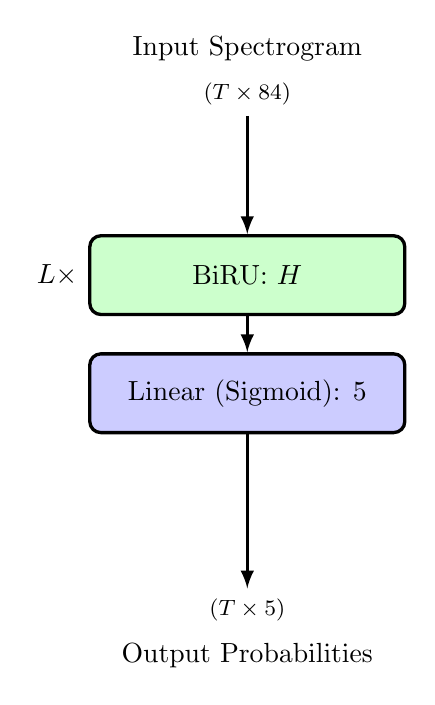
\begin{tikzpicture}[
    very thick,
    arrow/.style={
        -latex,
        very thick,
        rounded corners=0.2cm
    },
    ]

\node[anchor=south, label=above:{Input Spectrogram}] at (0, 0){\footnotesize{($T \times 84$)}};

\draw[arrow] (0, 0) -- (0, -1.5) node[rectangle, 
rounded corners, 
draw, 
anchor=north, 
label=west:$L\times$,
fill=green!20,
minimum height=1cm,
minimum width=4cm
] (a) {\acrshort{BiRU}: $H$};

\draw[arrow] (a) -- (0, -3) node[rectangle, 
rounded corners, 
draw, 
anchor=north, 
fill=blue!20,
minimum height=1cm,
minimum width=4cm
] (b) {Linear (Sigmoid): $5$};

\draw[arrow] (b) -- (0, -6);

\node[anchor=north, label=below:{Output Probabilities}] at (0, -6){\footnotesize{($T \times 5$)}};

\end{tikzpicture}
    \caption{RNN architecture structure.}
    \label{RNNFigure}
\end{figure}

\section{Convolutional Neural Network}

We've mentioned that spectrograms can be treated as images. Therefore it would make sense to try an image focused approach, by utilizing \textit{convolutions}. By applying convolutional layers, each timestep gets access to information around itself, a \textit{context}. These convolutional layers make up the primary building blocks for the \gls{CNN}.

\begin{figure}[H]
    \centering
    \begin{tikzpicture}[
    very thick,
    arrow/.style={
        -latex,
        very thick,
        rounded corners=0.2cm
    },
    ]

% ------ Grid ------

\draw[transform canvas={xscale=2}, step=0.25cm, ultra thin] (-2, 1) grid (2, 3);
\node[anchor=south] at (0, 3.25) {Contextual influence};
\node[anchor=east] at (-4, 2) {$D_\text{STFT}\times$};
\node[anchor=north] at (0, 0.75) {$T\times$};

% ------ Values ------

\fill[black!30] (-4.0, 1.0) rectangle (-3.5, 1.25);
\fill[black!30] (-3.5, 1.0) rectangle (-3.0, 1.25);
\fill[black!30] (-3.0, 1.0) rectangle (-2.5, 1.25);
\fill[black!30] (-2.5, 1.0) rectangle (-2.0, 1.25);
\fill[black!30] (-2.0, 1.0) rectangle (-1.5, 1.25);
\fill[black!30] (-1.5, 1.0) rectangle (-1.0, 1.25);
\fill[black!20] (-1.0, 1.0) rectangle (-0.5, 1.25);
\fill[black!20] (-0.5, 1.0) rectangle (0.0, 1.25);
\fill[black!20] (0.0, 1.0) rectangle (0.5, 1.25);
\fill[black!20] (0.5, 1.0) rectangle (1.0, 1.25);
\fill[black!20] (1.0, 1.0) rectangle (1.5, 1.25);
\fill[black!20] (1.5, 1.0) rectangle (2.0, 1.25);
\fill[black!20] (2.0, 1.0) rectangle (2.5, 1.25);
\fill[black!10] (2.5, 1.0) rectangle (3.0, 1.25);
\fill[black!20] (3.0, 1.0) rectangle (3.5, 1.25);
\fill[black!20] (3.5, 1.0) rectangle (4.0, 1.25);
\fill[black!40] (-4.0, 1.25) rectangle (-3.5, 1.5);
\fill[black!40] (-3.5, 1.25) rectangle (-3.0, 1.5);
\fill[black!40] (-3.0, 1.25) rectangle (-2.5, 1.5);
\fill[black!40] (-2.5, 1.25) rectangle (-2.0, 1.5);
\fill[black!30] (-2.0, 1.25) rectangle (-1.5, 1.5);
\fill[black!30] (-1.5, 1.25) rectangle (-1.0, 1.5);
\fill[black!30] (-1.0, 1.25) rectangle (-0.5, 1.5);
\fill[black!40] (-0.5, 1.25) rectangle (0.0, 1.5);
\fill[black!50] (0.0, 1.25) rectangle (0.5, 1.5);
\fill[black!50] (0.5, 1.25) rectangle (1.0, 1.5);
\fill[black!60] (1.0, 1.25) rectangle (1.5, 1.5);
\fill[black!50] (1.5, 1.25) rectangle (2.0, 1.5);
\fill[black!40] (2.0, 1.25) rectangle (2.5, 1.5);
\fill[black!40] (2.5, 1.25) rectangle (3.0, 1.5);
\fill[black!50] (3.0, 1.25) rectangle (3.5, 1.5);
\fill[black!50] (3.5, 1.25) rectangle (4.0, 1.5);
\fill[black!20] (-4.0, 1.5) rectangle (-3.5, 1.75);
\fill[black!20] (-3.5, 1.5) rectangle (-3.0, 1.75);
\fill[black!10] (-3.0, 1.5) rectangle (-2.5, 1.75);
\fill[black!10] (-2.5, 1.5) rectangle (-2.0, 1.75);
\fill[black!10] (-2.0, 1.5) rectangle (-1.5, 1.75);
\fill[black!10] (-1.5, 1.5) rectangle (-1.0, 1.75);
\fill[black!10] (-1.0, 1.5) rectangle (-0.5, 1.75);
\fill[black!20] (-0.5, 1.5) rectangle (0.0, 1.75);
\fill[black!30] (0.0, 1.5) rectangle (0.5, 1.75);
\fill[black!50] (0.5, 1.5) rectangle (1.0, 1.75);
\fill[black!60] (1.0, 1.5) rectangle (1.5, 1.75);
\fill[black!70] (1.5, 1.5) rectangle (2.0, 1.75);
\fill[black!60] (2.0, 1.5) rectangle (2.5, 1.75);
\fill[black!50] (2.5, 1.5) rectangle (3.0, 1.75);
\fill[black!40] (3.0, 1.5) rectangle (3.5, 1.75);
\fill[black!30] (3.5, 1.5) rectangle (4.0, 1.75);
\fill[black!10] (-4.0, 1.75) rectangle (-3.5, 2.0);
\fill[black!10] (-3.5, 1.75) rectangle (-3.0, 2.0);
\fill[black!10] (-3.0, 1.75) rectangle (-2.5, 2.0);
\fill[black!10] (-2.5, 1.75) rectangle (-2.0, 2.0);
\fill[black!10] (-2.0, 1.75) rectangle (-1.5, 2.0);
\fill[black!10] (-1.5, 1.75) rectangle (-1.0, 2.0);
\fill[black!10] (-1.0, 1.75) rectangle (-0.5, 2.0);
\fill[black!20] (-0.5, 1.75) rectangle (0.0, 2.0);
\fill[black!40] (0.0, 1.75) rectangle (0.5, 2.0);
\fill[black!50] (0.5, 1.75) rectangle (1.0, 2.0);
\fill[black!60] (1.0, 1.75) rectangle (1.5, 2.0);
\fill[black!60] (1.5, 1.75) rectangle (2.0, 2.0);
\fill[black!60] (2.0, 1.75) rectangle (2.5, 2.0);
\fill[black!60] (2.5, 1.75) rectangle (3.0, 2.0);
\fill[black!60] (3.0, 1.75) rectangle (3.5, 2.0);
\fill[black!60] (3.5, 1.75) rectangle (4.0, 2.0);
\fill[black!10] (-3.5, 2.0) rectangle (-3.0, 2.25);
\fill[black!10] (-1.0, 2.0) rectangle (-0.5, 2.25);
\fill[black!20] (-0.5, 2.0) rectangle (0.0, 2.25);
\fill[black!20] (0.0, 2.0) rectangle (0.5, 2.25);
\fill[black!20] (0.5, 2.0) rectangle (1.0, 2.25);
\fill[black!30] (1.0, 2.0) rectangle (1.5, 2.25);
\fill[black!30] (1.5, 2.0) rectangle (2.0, 2.25);
\fill[black!20] (2.0, 2.0) rectangle (2.5, 2.25);
\fill[black!20] (2.5, 2.0) rectangle (3.0, 2.25);
\fill[black!20] (3.0, 2.0) rectangle (3.5, 2.25);
\fill[black!30] (3.5, 2.0) rectangle (4.0, 2.25);
\fill[black!10] (-0.5, 2.25) rectangle (0.0, 2.5);
\fill[black!10] (0.0, 2.25) rectangle (0.5, 2.5);
\fill[black!10] (0.5, 2.25) rectangle (1.0, 2.5);
\fill[black!10] (1.0, 2.25) rectangle (1.5, 2.5);
\fill[black!10] (1.5, 2.25) rectangle (2.0, 2.5);
\fill[black!10] (2.0, 2.25) rectangle (2.5, 2.5);
\fill[black!10] (2.5, 2.25) rectangle (3.0, 2.5);
\fill[black!10] (3.0, 2.25) rectangle (3.5, 2.5);
\fill[black!10] (3.5, 2.25) rectangle (4.0, 2.5);

% ------ Outline ------
\draw[thick] (-4, 1) -- (4, 1) -- (4, 3) -- (-4, 3) -- cycle;

% ------ Influence ------

\draw[ultra thick, color=red, pattern=north east lines, pattern color=red] (-0.5, 1) -- (0, 1) -- (0, 3) -- (-0.5, 3) -- cycle;

\draw[thick, color=red] (-1, 1) -- (0.5, 1) -- (0.5, 3.) -- (-1, 3) -- cycle;


\end{tikzpicture}
    \caption{Visualization of a timestep's contextual influence with CNNs.}
    \label{CNNInfluenceFigure}
\end{figure}

\gls{CNN}s have been shown to give reasonable performance within \gls{ADT}. This could be due to contextual information being important for identifying instrument onsets, and making learning easier for our models~\cite{Vogl2017DrumTV}.

\subsection{Implementation}

Our \gls{CNN} architecure consists of $I \in \{1, 2, 3\}$ initial convolutional blocks. Inside this block, convolutional layers have an increasing number of kernels $C = \{32, 64, 96\}$, intuitively leading to an increase in complexity along with depth. Then we have a varying amount of fully connected layers $L \in \{1, 2, 3, 4\}$, projecting into a latent space sized $H \in \{72, 144, 288, 576\}$. And last, an output layer giving onset probabilities.

\begin{figure}[H]
    \centering
    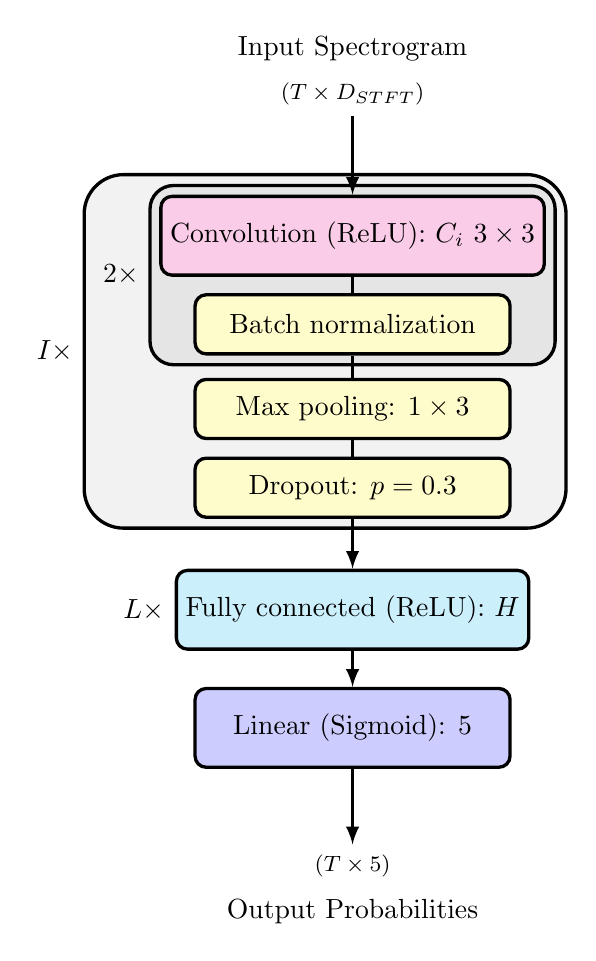
\begin{tikzpicture}[
    very thick,
    arrow/.style={
        -latex,
        very thick,
        rounded corners=0.2cm
    },
    ]

\node[anchor=south, label=above:{Input Spectrogram}] at (0, -0.5){\footnotesize{($T \times D_\text{STFT}$)}};

\draw[arrow] (0, -0.5) -- (0, -1.5) node [rectangle,
rounded corners,
draw,
anchor=north,
fill=magenta!20,
minimum height=1cm,
minimum width=4cm
] (a) {Convolution (ReLU): $C_i$  $3 \times 3$};

\draw (a) -- (0, -2.75) node[rectangle,
rounded corners,
draw,
anchor=north,
fill=yellow!20,
minimum height=0.75cm,
minimum width=4cm
] (b) {Batch normalization};

\draw (b) -- (0, -3.825) node[rectangle,
rounded corners,
draw,
anchor=north,
fill=yellow!20,
minimum height=0.75cm,
minimum width=4cm
] (c) {Max pooling: $1 \times 3$};

\draw (c) -- (0, -4.825) node[rectangle,
rounded corners,
draw,
anchor=north,
fill=yellow!20,
minimum height=0.75cm,
minimum width=4cm
] (d) {Dropout: $p = 0.3$};

\begin{scope}[on background layer]
    \node[rectangle,
    fill=gray!20,
    rounded corners=3mm,
    label={[name=ablabel]west:$2\times$},
    draw,
    very thick,
    fit=(a) (b)] (ab) {};
    \node[rectangle,
    fill=gray!10,
    rounded corners=5mm,
    label=west:$I\times$,
    draw,
    very thick,
    fit= (ab) (ablabel) (d)] {};
    \node[rectangle,
    fill=gray!20,
    rounded corners=3mm,
    label={[name=ablabel]west:$2\times$},
    draw,
    very thick,
    fit=(a) (b)] (ab) {};
\end{scope}


\draw[arrow] (d) -- (0, -6.25) node[rectangle, 
rounded corners, 
draw, 
anchor=north, 
label=west:$L\times$,
fill=cyan!20,
minimum height=1cm,
minimum width=4cm
] (g) {Fully connected (ReLU): $H$};

\draw[arrow] (g) -- (0, -7.75) node[rectangle, 
rounded corners, 
draw, 
anchor=north, 
fill=blue!20,
minimum height=1cm,
minimum width=4cm
] (h) {Linear (Sigmoid): $5$};

\draw[arrow] (h) -- (0, -9.75);

\node[anchor=north, label=below:{Output Probabilities}] at (0, -9.75){\footnotesize{($T \times 5$)}};

\end{tikzpicture}
    \caption{CNN architecture structure.}
    \label{CNNFigure}
\end{figure}

\section[Convolutional RNN]{Convolutional Recurrent Neural Network}

The previous features, recurrent layers and convolutions, are not mutually exclusive. Theoretically they can harmonize together, complementing eachother for easier learning. This results in the \gls{CRNN} architecture.

Intuitively, the \gls{CNN}s ability to process images like the spectrogram, together with the \gls{RNN}s ability to understand temporal sequence data should prove beneficial for \gls{ADT} tasks. And indeed, this combination of cross-timestep memory and contextual data representation has shown to be insightful~\cite{Vogl2017DrumTV, vogl2018multiinstrumentdrumtranscription, signals4040042}.

\begin{figure}[H]
    \centering
    \begin{tikzpicture}[
    very thick,
    arrow/.style={
        -latex,
        very thick,
        rounded corners=0.2cm
    },
    ]

% ------ Grid ------

\draw[transform canvas={xscale=2}, step=0.25cm, ultra thin] (-2, 1) grid (2, 3);
\node[anchor=south] at (0, 3.25) {Combinative influence};
\node[anchor=east] at (-4, 2) {$D_\text{STFT}\times$};
\node[anchor=north] at (0, 0.75) {$T\times$};

% ------ Values ------

\fill[black!30] (-4.0, 1.0) rectangle (-3.5, 1.25);
\fill[black!30] (-3.5, 1.0) rectangle (-3.0, 1.25);
\fill[black!30] (-3.0, 1.0) rectangle (-2.5, 1.25);
\fill[black!30] (-2.5, 1.0) rectangle (-2.0, 1.25);
\fill[black!30] (-2.0, 1.0) rectangle (-1.5, 1.25);
\fill[black!30] (-1.5, 1.0) rectangle (-1.0, 1.25);
\fill[black!20] (-1.0, 1.0) rectangle (-0.5, 1.25);
\fill[black!20] (-0.5, 1.0) rectangle (0.0, 1.25);
\fill[black!20] (0.0, 1.0) rectangle (0.5, 1.25);
\fill[black!20] (0.5, 1.0) rectangle (1.0, 1.25);
\fill[black!20] (1.0, 1.0) rectangle (1.5, 1.25);
\fill[black!20] (1.5, 1.0) rectangle (2.0, 1.25);
\fill[black!20] (2.0, 1.0) rectangle (2.5, 1.25);
\fill[black!10] (2.5, 1.0) rectangle (3.0, 1.25);
\fill[black!20] (3.0, 1.0) rectangle (3.5, 1.25);
\fill[black!20] (3.5, 1.0) rectangle (4.0, 1.25);
\fill[black!40] (-4.0, 1.25) rectangle (-3.5, 1.5);
\fill[black!40] (-3.5, 1.25) rectangle (-3.0, 1.5);
\fill[black!40] (-3.0, 1.25) rectangle (-2.5, 1.5);
\fill[black!40] (-2.5, 1.25) rectangle (-2.0, 1.5);
\fill[black!30] (-2.0, 1.25) rectangle (-1.5, 1.5);
\fill[black!30] (-1.5, 1.25) rectangle (-1.0, 1.5);
\fill[black!30] (-1.0, 1.25) rectangle (-0.5, 1.5);
\fill[black!40] (-0.5, 1.25) rectangle (0.0, 1.5);
\fill[black!50] (0.0, 1.25) rectangle (0.5, 1.5);
\fill[black!50] (0.5, 1.25) rectangle (1.0, 1.5);
\fill[black!60] (1.0, 1.25) rectangle (1.5, 1.5);
\fill[black!50] (1.5, 1.25) rectangle (2.0, 1.5);
\fill[black!40] (2.0, 1.25) rectangle (2.5, 1.5);
\fill[black!40] (2.5, 1.25) rectangle (3.0, 1.5);
\fill[black!50] (3.0, 1.25) rectangle (3.5, 1.5);
\fill[black!50] (3.5, 1.25) rectangle (4.0, 1.5);
\fill[black!20] (-4.0, 1.5) rectangle (-3.5, 1.75);
\fill[black!20] (-3.5, 1.5) rectangle (-3.0, 1.75);
\fill[black!10] (-3.0, 1.5) rectangle (-2.5, 1.75);
\fill[black!10] (-2.5, 1.5) rectangle (-2.0, 1.75);
\fill[black!10] (-2.0, 1.5) rectangle (-1.5, 1.75);
\fill[black!10] (-1.5, 1.5) rectangle (-1.0, 1.75);
\fill[black!10] (-1.0, 1.5) rectangle (-0.5, 1.75);
\fill[black!20] (-0.5, 1.5) rectangle (0.0, 1.75);
\fill[black!30] (0.0, 1.5) rectangle (0.5, 1.75);
\fill[black!50] (0.5, 1.5) rectangle (1.0, 1.75);
\fill[black!60] (1.0, 1.5) rectangle (1.5, 1.75);
\fill[black!70] (1.5, 1.5) rectangle (2.0, 1.75);
\fill[black!60] (2.0, 1.5) rectangle (2.5, 1.75);
\fill[black!50] (2.5, 1.5) rectangle (3.0, 1.75);
\fill[black!40] (3.0, 1.5) rectangle (3.5, 1.75);
\fill[black!30] (3.5, 1.5) rectangle (4.0, 1.75);
\fill[black!10] (-4.0, 1.75) rectangle (-3.5, 2.0);
\fill[black!10] (-3.5, 1.75) rectangle (-3.0, 2.0);
\fill[black!10] (-3.0, 1.75) rectangle (-2.5, 2.0);
\fill[black!10] (-2.5, 1.75) rectangle (-2.0, 2.0);
\fill[black!10] (-2.0, 1.75) rectangle (-1.5, 2.0);
\fill[black!10] (-1.5, 1.75) rectangle (-1.0, 2.0);
\fill[black!10] (-1.0, 1.75) rectangle (-0.5, 2.0);
\fill[black!20] (-0.5, 1.75) rectangle (0.0, 2.0);
\fill[black!40] (0.0, 1.75) rectangle (0.5, 2.0);
\fill[black!50] (0.5, 1.75) rectangle (1.0, 2.0);
\fill[black!60] (1.0, 1.75) rectangle (1.5, 2.0);
\fill[black!60] (1.5, 1.75) rectangle (2.0, 2.0);
\fill[black!60] (2.0, 1.75) rectangle (2.5, 2.0);
\fill[black!60] (2.5, 1.75) rectangle (3.0, 2.0);
\fill[black!60] (3.0, 1.75) rectangle (3.5, 2.0);
\fill[black!60] (3.5, 1.75) rectangle (4.0, 2.0);
\fill[black!10] (-3.5, 2.0) rectangle (-3.0, 2.25);
\fill[black!10] (-1.0, 2.0) rectangle (-0.5, 2.25);
\fill[black!20] (-0.5, 2.0) rectangle (0.0, 2.25);
\fill[black!20] (0.0, 2.0) rectangle (0.5, 2.25);
\fill[black!20] (0.5, 2.0) rectangle (1.0, 2.25);
\fill[black!30] (1.0, 2.0) rectangle (1.5, 2.25);
\fill[black!30] (1.5, 2.0) rectangle (2.0, 2.25);
\fill[black!20] (2.0, 2.0) rectangle (2.5, 2.25);
\fill[black!20] (2.5, 2.0) rectangle (3.0, 2.25);
\fill[black!20] (3.0, 2.0) rectangle (3.5, 2.25);
\fill[black!30] (3.5, 2.0) rectangle (4.0, 2.25);
\fill[black!10] (-0.5, 2.25) rectangle (0.0, 2.5);
\fill[black!10] (0.0, 2.25) rectangle (0.5, 2.5);
\fill[black!10] (0.5, 2.25) rectangle (1.0, 2.5);
\fill[black!10] (1.0, 2.25) rectangle (1.5, 2.5);
\fill[black!10] (1.5, 2.25) rectangle (2.0, 2.5);
\fill[black!10] (2.0, 2.25) rectangle (2.5, 2.5);
\fill[black!10] (2.5, 2.25) rectangle (3.0, 2.5);
\fill[black!10] (3.0, 2.25) rectangle (3.5, 2.5);
\fill[black!10] (3.5, 2.25) rectangle (4.0, 2.5);

% ------ Outline ------
\draw[thick] (-4, 1) -- (4, 1) -- (4, 3) -- (-4, 3) -- cycle;

% ------ Influence ------

\draw[ultra thick, color=red, pattern=north east lines, pattern color=red] (-0.5, 0.75) -- (0, 0.75) -- (0, 3.25) -- (-0.5, 3.25) -- cycle;
\draw[very thick, color=red] (-1, 0.75) -- (0.5, 0.75) -- (0.5, 3.25) -- (-1, 3.25) -- cycle;

\draw[thick, color=red, pattern=north east lines, pattern color=red] (-1, 0.875) -- (-0.5, 0.875) -- (-0.5, 3.125) -- (-1, 3.125) -- cycle;
\draw[thin, color=red] (-1.5, 0.875) -- (-1, 0.875) -- (-1, 3.125) -- (-1.5, 3.125) -- cycle;
\draw[thick, color=red, pattern=north east lines, pattern color=red] (0, 0.875) -- (0.5, 0.875) -- (0.5, 3.125) -- (0, 3.125) -- cycle;
\draw[thin, color=red] (0.5, 0.875) -- (1.0, 0.875) -- (1.0, 3.125) -- (0.5, 3.125) -- cycle;

\draw[very thin, color=red, pattern=north east lines, pattern color=red] (-1.5, 0.95) -- (-1, 0.95) -- (-1, 3.05) -- (-1.5, 3.05) -- cycle;
\draw[ultra thin, color=red] (-2, 0.95) -- (-1.5, 0.95) -- (-1.5, 3.05) -- (-2, 3.05) -- cycle;
\draw[very thin, color=red, pattern=north east lines, pattern color=red] (0.5, 0.95) -- (1, 0.95) -- (1, 3.05) -- (0.5, 3.05) -- cycle;
\draw[ultra thin, color=red] (1, 0.95) -- (1.5, 0.95) -- (1.5, 3.05) -- (1, 3.05) -- cycle;


\end{tikzpicture}
    \caption{Visualization of a timestep's contextual and cross-timestep influence with CRNNs.}
    \label{CRNNInfluenceFigure}
\end{figure}

\subsection{Implementation}

We begin with a fixed-size convolutional block with $I = 2$, as used by several \gls{ADT} authors~\cite{Vogl2017DrumTV, signals4040042}. Following the \gls{CNN} it has an increasing number of kernels $C = \{32, 64\}$. We then, similar to the \gls{RNN}, have a \gls{BiRU} layer of either a \gls{GRU} or \gls{LSTM}, with number of layers $L \in \{2, 3, 4, 5\}$ and hidden size $H \in \{72, 144, 288\}$.

\begin{figure}[H]
    \centering
    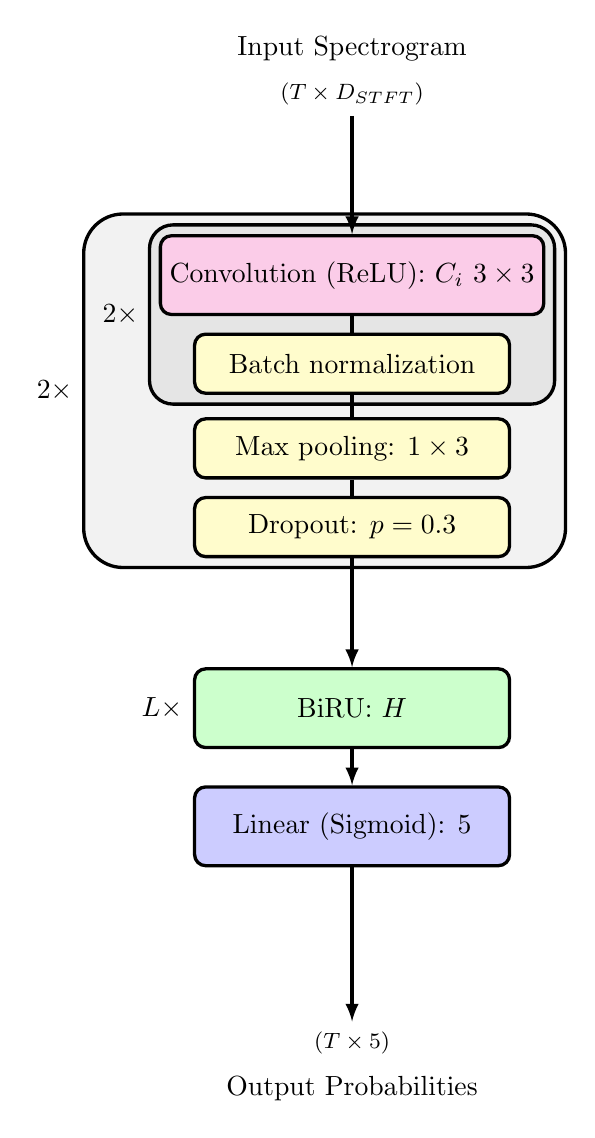
\begin{tikzpicture}[
    very thick,
    arrow/.style={
        -latex,
        very thick,
        rounded corners=0.2cm
    },
    ]

\node[anchor=south, label=above:{Input Spectrogram}] at (0, 0){\footnotesize{($T \times D_\text{STFT}$)}};

\draw[arrow] (0, 0) -- (0, -1.5) node [rectangle,
rounded corners,
draw,
anchor=north,
fill=magenta!20,
minimum height=1cm,
minimum width=4cm
] (a) {Convolution (ReLU): $C_i$  $3 \times 3$};

\draw (a) -- (0, -2.75) node[rectangle,
rounded corners,
draw,
anchor=north,
fill=yellow!20,
minimum height=0.75cm,
minimum width=4cm
] (b) {Batch normalization};

\draw (b) -- (0, -3.825) node[rectangle,
rounded corners,
draw,
anchor=north,
fill=yellow!20,
minimum height=0.75cm,
minimum width=4cm
] (c) {Max pooling: $1 \times 3$};

\draw (c) -- (0, -4.825) node[rectangle,
rounded corners,
draw,
anchor=north,
fill=yellow!20,
minimum height=0.75cm,
minimum width=4cm
] (d) {Dropout: $p = 0.3$};

\begin{scope}[on background layer]
    \node[rectangle,
    fill=gray!20,
    rounded corners=3mm,
    label={[name=ablabel]west:$2\times$},
    draw,
    very thick,
    fit=(a) (b)] (ab) {};
    \node[rectangle,
    fill=gray!10,
    rounded corners=5mm,
    label=west:$2\times$,
    draw,
    very thick,
    fit= (ab) (ablabel) (d)] {};
    \node[rectangle,
    fill=gray!20,
    rounded corners=3mm,
    label={[name=ablabel]west:$2\times$},
    draw,
    very thick,
    fit=(a) (b)] (ab) {};
\end{scope}

\draw[arrow] (d) -- (0, -7) node[rectangle, 
rounded corners, 
draw, 
anchor=north, 
label=west:$L\times$,
fill=green!20,
minimum height=1cm,
minimum width=4cm
] (g) {BiRU: $H$};

\draw[arrow] (g) -- (0, -8.5) node[rectangle, 
rounded corners, 
draw, 
anchor=north, 
fill=blue!20,
minimum height=1cm,
minimum width=4cm
] (h) {Linear (Sigmoid): $5$};

\draw[arrow] (h) -- (0, -11.5);

\node[anchor=north, label=below:{Output Probabilities}] at (0, -11.5){\footnotesize{($T \times 5$)}};

\end{tikzpicture}
    \caption{Convolutional RNN architecture structure.}
    \label{CRNNFigure}
\end{figure}

\section{Convolutional Transformer}

Google's "Attention Is All You Need"~\cite{NIPS2017_3f5ee243} made headway in regards to sequence prediction. It introduced the \textit{Attention} layer, making a model capable of learning to \textit{attend} to different elements in a sequence, and learning the relationship between them. Models dropping the recurrent units in favour of attention blocks are called \textit{transformers}.

As mentioned, the \gls{RNN} displays difficulty in sustaining long range dependencies through its hidden state, and information further away tends to become attenuated. The attention layer solves this by allowing each element to individually attend to each other element in the sequence separately. Intuitively, it allows each element to \textit{"intelligently"} pick and choose where it wants to look, and what elements it wants to be influenced by. This stands in contrast to the recurrent units, where each element has to learn and predict what information about itself other elements could find useful, and \textit{"remembering"} that, adding it to the hidden state.

\textcolor{red}{Visualization of attention.}

Recently, the attention layers have shown great success in \gls{AMT} and \gls{ADT} tasks, in some cases proving superior to the \gls{RNN}~\cite{gardner2022mt3multitaskmultitrackmusic, chang2024yourmt3multiinstrumentmusictranscription, zehren2024analyzingreducingsynthetictorealtransfer}.

Simply replacing the recurrent layers with attention blocks could allow our model to reap the reward by increasing its ability to understand sequences, while keeping the previously gotten gains from the convolutional layer. Both inside and outside of \gls{ADT}, combining convolutional layers with transformers has seemed beneficial~\cite{zehren2024analyzingreducingsynthetictorealtransfer, gulati2020conformerconvolutionaugmentedtransformerspeech}.

\subsection{Implementation}

Similar to the \gls{CRNN}, an initial fixed-size convolutional block with $I = 2$ is used, with an increasing number of kernels $C = \{32, 64\}$. Then, we project the resulting latent space into a separate embedding dimension $D_e \in \{72, 144, 288\}$, before combining it with a sinusoidal positional encoding. 

Following this, the model contains $L \in \{2, 4, 6, 8\}$ standard pre-layer normalization attention block, as these recently have been shown to be more stable during learning than the post-layer versions~\cite{pmlr-v119-xiong20b}. These attention blocks contain multihead self-attention layers with $H \in \{2, 4, 6, 8\}$ number of heads.

\begin{figure}[H]
    \centering
    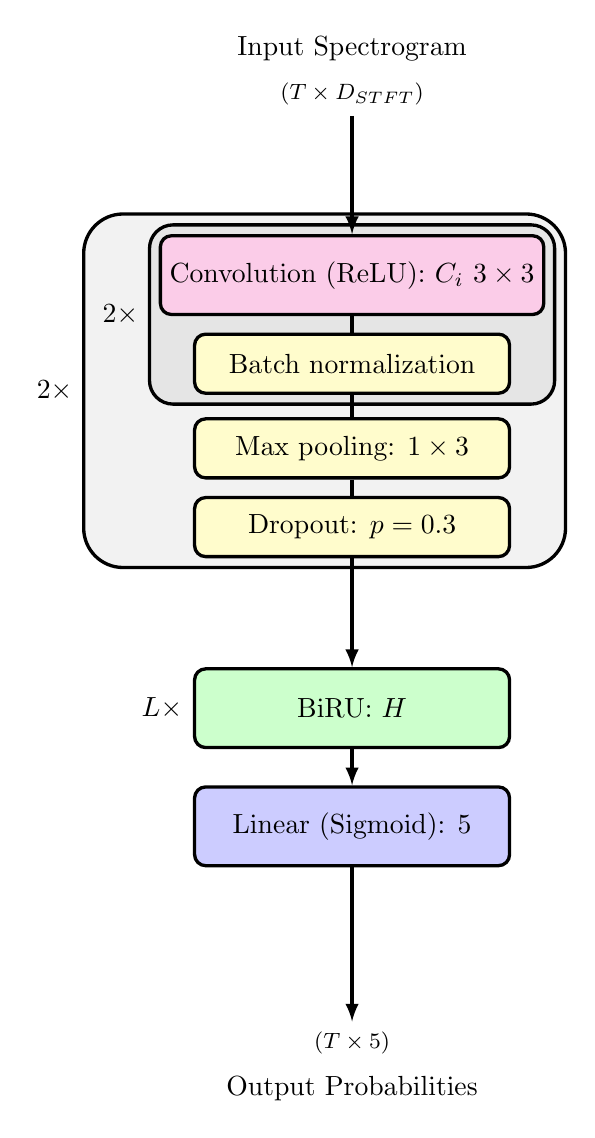
\begin{tikzpicture}[
    very thick,
    arrow/.style={
        -latex,
        very thick,
        rounded corners=0.2cm
    },
    ]

\node[anchor=south, label=above:{Input Spectrogram}] at (0, 0){\footnotesize{($T \times D_\text{STFT}$)}};

\draw[arrow] (0, 0) -- (0, -1.5) node [rectangle,
rounded corners,
draw,
anchor=north,
fill=magenta!20,
minimum height=1cm,
minimum width=4cm
] (a) {Convolution (ReLU): $C_i$  $3 \times 3$};

\draw (a) -- (0, -2.75) node[rectangle,
rounded corners,
draw,
anchor=north,
fill=yellow!20,
minimum height=0.75cm,
minimum width=4cm
] (b) {Batch normalization};

\draw (b) -- (0, -3.825) node[rectangle,
rounded corners,
draw,
anchor=north,
fill=yellow!20,
minimum height=0.75cm,
minimum width=4cm
] (c) {Max pooling: $1 \times 3$};

\draw (c) -- (0, -4.825) node[rectangle,
rounded corners,
draw,
anchor=north,
fill=yellow!20,
minimum height=0.75cm,
minimum width=4cm
] (d) {Dropout: $p = 0.3$};

\begin{scope}[on background layer]
    \node[rectangle,
    fill=gray!20,
    rounded corners=3mm,
    label={[name=ablabel]west:$2\times$},
    draw,
    very thick,
    fit=(a) (b)] (ab) {};
    \node[rectangle,
    fill=gray!10,
    rounded corners=5mm,
    label=west:$2\times$,
    draw,
    very thick,
    fit= (ab) (ablabel) (d)] {};
    \node[rectangle,
    fill=gray!20,
    rounded corners=3mm,
    label={[name=ablabel]west:$2\times$},
    draw,
    very thick,
    fit=(a) (b)] (ab) {};
\end{scope}

\draw[arrow] (d) -- (0, -7) node[rectangle, 
rounded corners, 
draw, 
anchor=north, 
label=west:$L\times$,
fill=green!20,
minimum height=1cm,
minimum width=4cm
] (g) {BiRU: $H$};

\draw[arrow] (g) -- (0, -8.5) node[rectangle, 
rounded corners, 
draw, 
anchor=north, 
fill=blue!20,
minimum height=1cm,
minimum width=4cm
] (h) {Linear (Sigmoid): $5$};

\draw[arrow] (h) -- (0, -11.5);

\node[anchor=north, label=below:{Output Probabilities}] at (0, -11.5){\footnotesize{($T \times 5$)}};

\end{tikzpicture}
    \caption{Convolutional RNN architecture structure.}
    \label{CRNNFigure}
\end{figure}

\section{Vision Transformer}